\documentclass[10pt, conference, compsocconf]{IEEEtran}
% Add the compsocconf option for Computer Society conferences.
%
% If IEEEtran.cls has not been installed into the LaTeX system files,
% manually specify the path to it like:
% \documentclass[conference]{../sty/IEEEtran}
\usepackage{cite}

\usepackage[cmex10]{amsmath}
\usepackage{amssymb}

\usepackage{algorithm}
\usepackage{array}
\usepackage{algpseudocode}
\usepackage{indentfirst}
\usepackage[pdftex]{graphicx}
\usepackage[tight,footnotesize]{subfigure}


%\usepackage{algorithmic}


\begin{document}

\title{Evaluation of Design Trade-offs for Adders\\ in Approximate Datapath}
%Evaluation of Design Trade-offs for Approximate Arithmetic Operators
%Evaluation of Optimum Arithmetic Operators For Approximate Datapath Design

\author{\IEEEauthorblockN{Kan Shi and George A. Constantinides}
\IEEEauthorblockA{Department of Electrical and Electronic Engineering\\
Imperial College London\\
London, UK\\
Email: \{k.shi11, g.contantinides\}@imperial.ac.uk}
%\and
%\IEEEauthorblockN{Authors Name/s per 2nd Affiliation (Author)}
%\IEEEauthorblockA{line 1 (of Affiliation): dept. name of organization\\
%line 2: name of organization, acronyms acceptable\\
%line 3: City, Country\\
%line 4: Email: name@xyz.com}
}


\maketitle


\begin{abstract}
Releasing the stringent accuracy requirement would potentially offer greater freedom to create a design with better performance or energy efficiency. In this paper, we evaluate the design trade-offs for adders, which are key building blocks for many applications. We demonstrate the optimum design metric for adders, under the consideration of various design constraints, such as accuracy, operating frequency, silicon area, different types of adder structure and even alternative form of computer arithmetic for adder implementation. Two design scenarios are compared: one is the conventional design scenario where timing closure is met by adjusting operand word-lengths. The other is an overclocking scenario where timing violations are allowed to occur. We show that applying the overclocking approach to ripple carry adders can be more beneficial than using fast adders to achieve similar latency, because the worst cases only happen with very small probabilities. We also show that using the conventional approach on adders with new form of computer arithmetic is optimal for a wide range of design constraints. 

%We show that instead of losing precision to ensure timing closure, allowing timing violations to happen can be beneficial, because the worst case scenario only happens with a very small probability. 


\end{abstract}

\begin{IEEEkeywords}
approximate computing; adder; overclocking; online arithmetic;

\end{IEEEkeywords}


\section{Introduction}
Circuit performance has been increased tremendously over the past decades. However, in recent years people have observed an end of performance improvement [xx] due to the scaling of CMOS technology to the nanometer regime. In order to boost circuit performance, two standard design techniques are commonly adopted: one is to heavily pipeline the datapath, the other is to reduce the design precision. For the first technique, pipelining can be used to increase operating frequency, whereas the overall computational latency will not be affected. Therefore the application of this technique is limited in many embedded applications, which are often designed with strict latency specifications. The second technique is common especially with FPGA technology, which embodies the flexibility to implement customized variable representation and is able to optimize the operand word-length across the entire datapath to meet a given performance and area constraint. However, the precision loss will inevitably introduce quantization errors into the design.

Unfortunately, in both cases circuits are designed for the worst cases. In order to avoid potential timing violations, timing analysis tools tend to provide a more conservative path delay by adding guard bands and timing margins. However, continuing with this approach will become increasing expensive and difficult as technology shrinks.

To tackle this problem, a large volume of research activities were focused on the design methodology of relaxing the $100\%$ accuracy requirements and design constraints, while evaluating the corresponding design benefits and costs. Studies have shown that computing approximately provides extra opportunities to design circuits with better performance and less energy consumption. A brief discussion of the work in this area is given in Section~\ref{sec:Background}.

In this paper, we provide a detailed evaluation of design trade-offs for adders, which are key arithmetic primitives for a broad range of applications.

\section{Background}\label{sec:Background}
\subsection{Approximate Datapath Design}
Typically this can be achieved by either reducing the supply voltage [xxx] or increasing the operating frequency beyond the rated value [xxx].

\subsection{Online Arithmetic}

As an alternative form of computer arithmetic, online arithmetic has been used in numerous applications such as signal processing and control algorithms~\cite{Online_FPGADSP,Online_Control}. Online arithmetic was originally designed for digit-serial operation, as illustrated in Fig~\ref{Fig:OnlineDataFlow}. It can be seen that in order to generate the first output digit, $\delta$ digits of inputs are required, where $\delta$ is called the ``online delay''. $\delta$ is normally a small constant, which is independent of the precision. For ease of discussion, for the rest of this paper, the input data is assumed to be fixed point numbers in the range $(-1,1)$. Based on this premise, the online representation of $N$-digit operands and result at iteration $j$ are given by (\ref{Eq:Online_Operands}), where $j\in[-\delta,N-1]$ and $r$ denotes the radix \cite{Ercegovac_Book}.
%
\begin{figure}[tbp]
  \centering
  %\vspace{-2.5ex}
  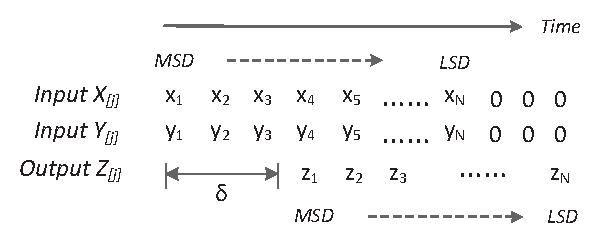
\includegraphics[width=.42\textwidth]{./figures/OnlineArithmetic_DataFlow.eps}
  %\vspace{-1ex}
  \caption{Dataflow in digit-serial online arithmetic, in which both inputs and outputs are processed from the MSD to the LSD. $\delta$ denotes the online delay.}
  \vspace{-2ex}
  \label{Fig:OnlineDataFlow}
\end{figure}
%
\begin{eqnarray}\label{Eq:Online_Operands}
\footnotesize
  X_{[j]}=\sum_{i=1}^{j+\delta}x_ir^{-i},~Y_{[j]}=\sum_{i=1}^{j+\delta}y_ir^{-i},~Z_{[j]}=\sum_{i=1}^{j}z_ir^{-i}
\normalsize
\end{eqnarray}

MSD-first operation is possible only if a redundant number system is used. Normally there are two most commonly used redundant number representations: carry-save (CS) \cite{CSadder} and signed-digit (SD) \cite{RedundantNumber}. With SD representation, each digit is represented using a redundant digit set $\{-a, \cdots,-1,0, 1, \cdots, a\}$, where $a\in[r/2,r-1]$. In comparison, the standard non-redundant representation only uses a digit set $\{0,\cdots,r-1\}$. Thus a standard number corresponds to several possible redundant representations. For example, the binary number $0.011$ can be represented in SD form as $0.1\overline{1}1$, $0.10\overline{1}$ or $0.011$ among many other possible representations.

Due to the redundancy, the MSDs of the result can be calculated using partial information from both inputs. Then the value of the number can be revised using the subsequent digits, because each number has multiple representations.

\section{Design Trade-offs of Different Adder Structures}
\subsection{Ripple Carry Adder}
Adders serve as a key building block for arithmetic operations. In general, the ripple carry adder (RCA) is the most straightforward and widely used adder structure. As such, in our previous work we proposed probabilistic models of overclocking errors for RCA.

For an $n$-bit RCA, it is composed of $n$ serial-connected full adders (FA). Typically the maximum frequency of RCA is determined by the longest carry propagation. Under the assumption that the carry propagation delay of each FA is a constant value $\mu$, the critical path of the RCA is: $\mu_{RCA}=n\mu$. For the sampling period $T_S$, it follows that if $T_S\geqslant\mu_{RCA}$, correct result will always be sampled; otherwise if $T_S<\mu_{RCA}$, intermediate be sampled and potentially generating errors. In the previous work, the mean value of overclocking error is modeled as given in (\ref{Eq:MeanError_RCA}), where coefficient $b$ is given in (\ref{Eq:b}) and it determines the maximum length of error-free carry propagation in bits.
%
\begin{eqnarray}\label{Eq:MeanError_RCA}
    E_O=\left\{
        \begin{matrix}
            2^{-b}-2^{-n-1}, & \textrm{if $b\leq n$}\\
            0, & \textrm{otherwise}
        \end{matrix}
        \right.
\end{eqnarray}
%
\begin{eqnarray}\label{Eq:b}
    b:=\left\lceil \frac{T_S}{\mu} \right\rceil=\left\lceil \frac{1}{\mu\cdot f_S}\right\rceil
\end{eqnarray}

On the other hand, a specific timing target can be met by truncating the word-length of RCA while timing violation is not permitted. This will result in truncation error for most data.  The mean value of truncation error is also modeled as given in~(\ref{Eq:MeanTruncError_RCA}) [xxx], where parameters $k$ and $n$ denote the word-length of RCA before and after truncation, respectively. 
%
\begin{eqnarray}\label{Eq:MeanTruncError_RCA}
    E_O=\left\{
        \begin{matrix}
            2^{-n}-2^{-k}, & \textrm{if $n<k$}\\
            0, & \textrm{otherwise}
        \end{matrix}
        \right.
\end{eqnarray}

In this paper we consider two design scenarios for RCA: one is the overclocking scenario where timing violation is allowed to happen while maintaining the original word-length; the other is the trad scenario by truncating RCA word-length to meet timing. For a given $f_S$, in the first design scenario we have $n=k$. In the second design scenario we have $n=b-1$ to prevent timing violation while minimizing the value of $E_O$. Therefore the comparison between the two scenarios in mean error value is given in (\ref{Eq:ErrorCompare_RCA}) by updating (\ref{Eq:MeanError_RCA}) and (\ref{Eq:MeanTruncError_RCA}) respectively. As seen in (\ref{Eq:ErrorCompare_RCA}), in theory the mean value of error in the overclocking scenario ($E_{oc}$) is two times smaller than that in the traditional scenario ($E_{trad}$).
%
\begin{eqnarray}\label{Eq:ErrorCompare_RCA}
    \frac{E_{oc}}{E_{trad}} = \frac{2^{-b}-2^{-n-1}|_{n=k}}{2^{-n}-2^{-k}|_{n=b-1}}=\frac{1}{2}
\end{eqnarray}

\subsection{Carry Select Adder}
Although smaller value of mean error can be achieved in the overclocking scenario, it costs extra area because the full precision is maintained. Instead, alternative adder structures, such as carry select adder (CSA), are originally designed to trade silicon area for low latency. In a CSA, the carry chain is divided into multiple overlapped stages, and each stage contains two RCAs and two multiplexers, as shown in Fig. xxx(a) and Fig. xxx(b). For a given input, two additions are performed simultaneously within a single stage where the carry input is zero and one separately. One of these two results is then selected according to the actual carry input. Although this structure brings performance benefits, it costs extra hardware resources compared to a standard RCA because the carry chain is duplicated. Furthermore, multiplexers are area-expensive to implement with FPGA technology.

%In this paper, we take CSA with different stages into comparison when considering a variety of accuracy, performance and area trade-offs. The results are shown in Section.xxx. 

\subsection{Online Adder}\label{subsec:online_adder}
%\subsubsection{Structure}
In addition to standard binary arithmetic, alternative forms of computer arithmetic was studied to boost performance. For example, adder with online arithmetic is also designed for low latency at the cost of more silicon area. The structure of a digit-parallel online adder (OA) where all signals represented with SD numbers of digit set $\{-1,0,1\}$ is shown in Fig.~\ref{Fig:Radix2SD_adder}. The module ``3:2'' denotes a 3:2 compressor, which takes three inputs and generates two outputs, and is logically equivalent to a full adder (FA). A major advantage of the redundant number system over the standard ripple-carry based arithmetic is that the propagation of carry is eliminated, resulting in a precision-independent computation time for addition. As labelled in Fig.~\ref{Fig:Radix2SD_adder}, ideally the computation delay of this adder is only two FA delays for any operand word-length, at the expenses of one extra FA for each digit of operands. 
%
\begin{figure}[tbp]
  \centering
  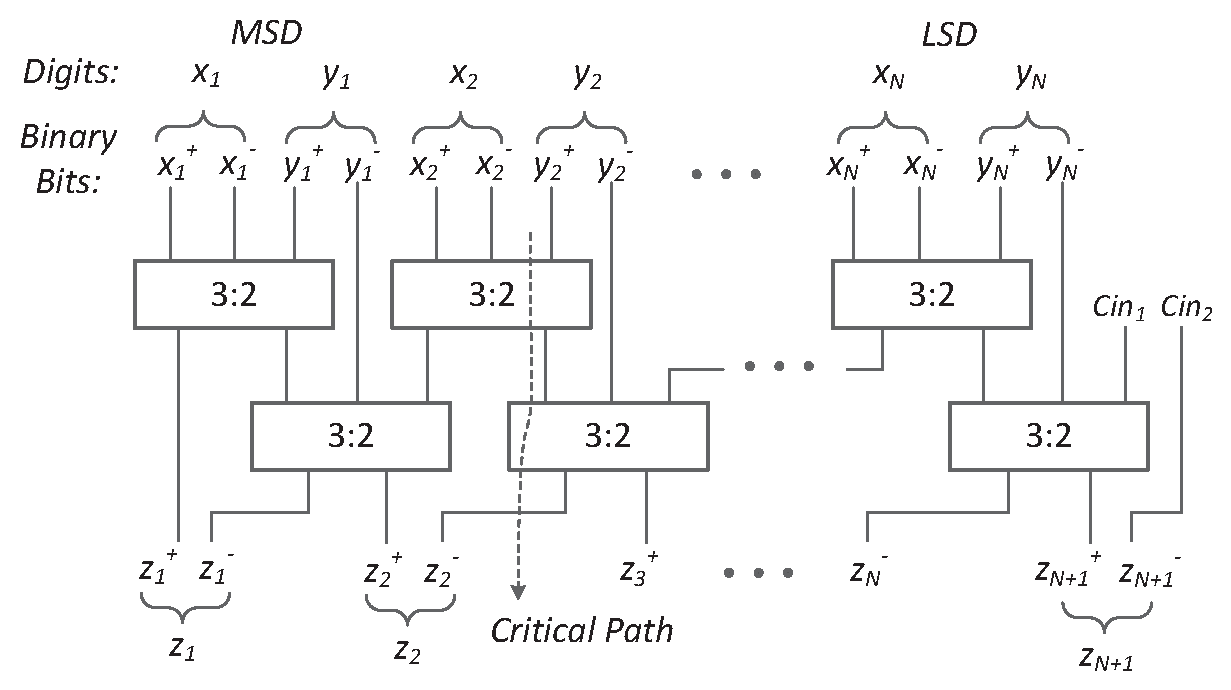
\includegraphics[width=.45\textwidth]{./figures/SDAdder.eps}
  \caption{An $N$-digit binary digit-parallel online adder. Both inputs and outputs are represented using SD representation. ``3:2'' denotes a 3:2 compressor.}
  \label{Fig:Radix2SD_adder}
\end{figure}

\subsection{Design Trade-offs for Adders}
In this section, we initially demonstrate the benefits of CSA and OA in accuracy and performance, as well as the area overhead in comparison to RCA. As an example, the maximum word-lengths with respect to a variety of operating frequencies for RCA, CSA and OA are illustrated in Fig.~\ref{Fig:max_wl_adder}, where overclocking error is not allowed to happen and the conventional design scenario is evaluated for all structures. Also notice that in the experiment we consider the word-length of adders from 4-bit to 32-bit with a step of 4-bit. For a finer grain experiment, the trend will be similar to that in Fig.~\ref{Fig:max_wl_adder}.
%
\begin{figure}[tbp]
  \centering
  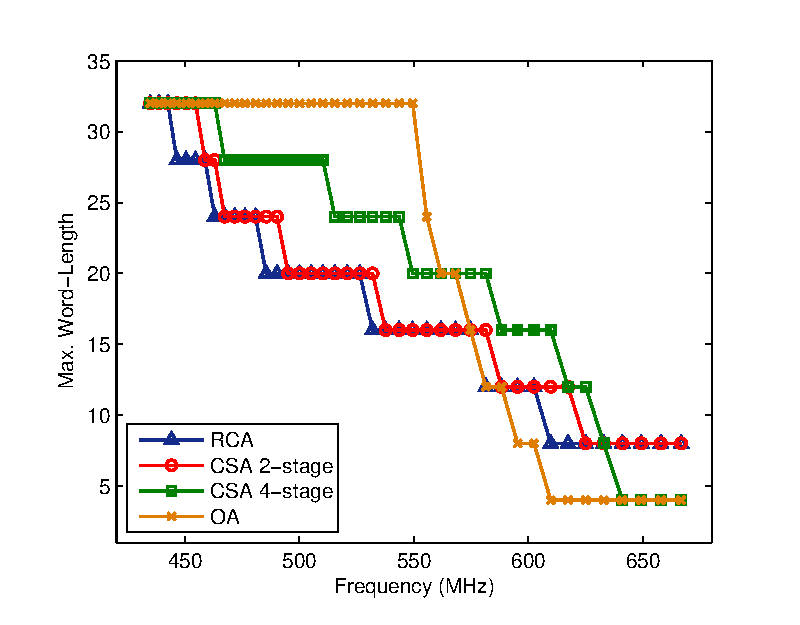
\includegraphics[width=.5\textwidth]{./figures/exp/max_wl.eps}
  \vspace{-4ex}
  \caption{The maximum word-lengths of different adder structures with respect to a variety of frequencies. The results are obtained from Xilinx ISE 14.7.}
  \label{Fig:max_wl_adder}
\end{figure}

As can be seen in Fig.~\ref{Fig:max_wl_adder}, for a relatively relaxed frequency requirement, both CSA and OA can be implemented with greater word-lengths than RCA. For CSA, this is because the stage parallelism enables a larger word-length, even though the multiplexer delay limits the word-length of each stage in the CSA in comparison to RCA. For OA, an even larger gap in word-length can be observed when compared to RCA. Additionally, unlike RCA and CSA of which the word-length drops gradually with the increment of frequency, OA maintains the full precision across a large rang of frequencies. This is expected, because the critical path delay of OA is theoretically irrelevant to the operand word-length. However, we also observe that for a large frequency requirement, the word-length of OA drops drastically, while RCA and CSA with 2 stages outperform. This is because the multiplexer delay becomes comparable to the delay of the carry chain for CSA, and it inhibits the benefits of parallelism. 

We also record the corresponding area consumed by each adder structure in terms of look-up-tables (LUTs) in FPGA as depicted in Fig.~\ref{Fig:area_adder}. It can be seen that for a given frequency, CSA costs up to $4.5\times$ (4 stages) and $3.1\times$ (2 stages) area than RCA, and OA is up to $3.8\times$ larger than RCA for some frequency values. Therefore, we incorporate silicon area as another design metric besides accuracy and performance, and evaluate the optimum adder structure under various design trade-offs. In this paper, we examine both the overclocking scenario and the conventional scenario for RCA, while only considering the conventional scenario for other adder structures.
%
\begin{figure}[tbp]
  \centering
  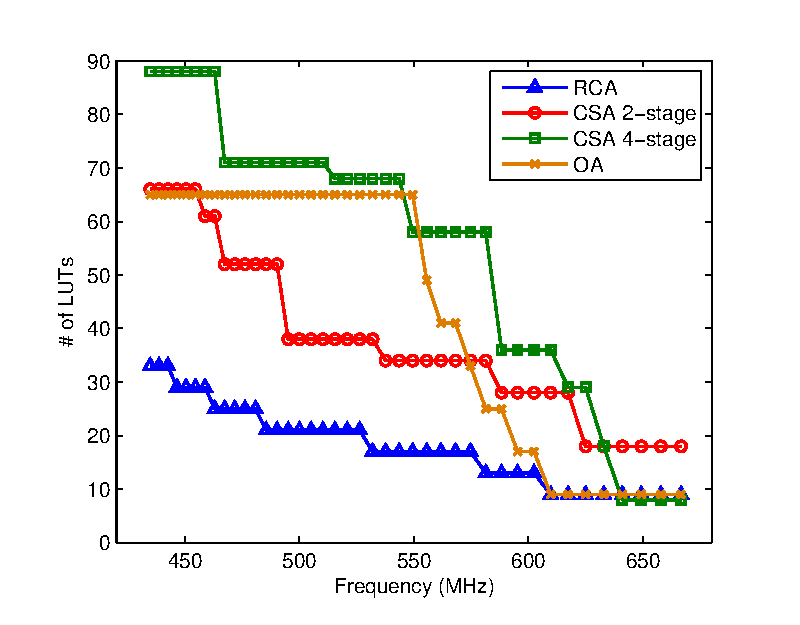
\includegraphics[width=.5\textwidth]{./figures/exp/area_adders.eps}
  \caption{The maximum word-length of different adder structures.}
  \label{Fig:area_adder}
\end{figure}



\section{Evaluation of Optimum Adder Structure}
In general, the evaluation could be of interest to a circuit designer in several ways. For example, suppose the algorithm designer wish the circuit to run at a given frequency within a given area budget, while achieving the minimum output error. Besides, for many applications, the circuit design would wish the circuit to operate as fast as possible with the minimum resource usage, whilst a certain error budget can be tolerated. In both cases, decisions must then be made on which adder structure achieves this minimum, and whether the circuit should be overclocked. 

\subsection{Optimum Adder Design Metric with Given Frequency and Area Requirements}
For this type of applications, the available area and expected operating frequency are given at the design time. As an example slice through the design space, in Fig.~\ref{Fig:Error_Area} we record the mean relative error (MRE) with respect to a range of operating frequencies for different design scenarios, when the area budget is set to 35 LUTs and 55 LUTs separately. MRE can be calculated as given by (\ref{Eq:MRE}), where $E_{error}$ and $E_{out}$ denote the mean value of error and the mean value of correct outputs, respectively. Notice that the optimum adder design metric that achieves the minimum error at outputs is labeled. 
%
\begin{eqnarray}\label{Eq:MRE}
  MRE=\frac{E_{error}}{E_{out}}\times100\%
\end{eqnarray}

\begin{figure}[tbp]
  %\vspace{-2ex}
  \centering
  \subfigure[Available LUT=35.]{
  \begin{minipage}[c]{0.5\textwidth}
    \centering
    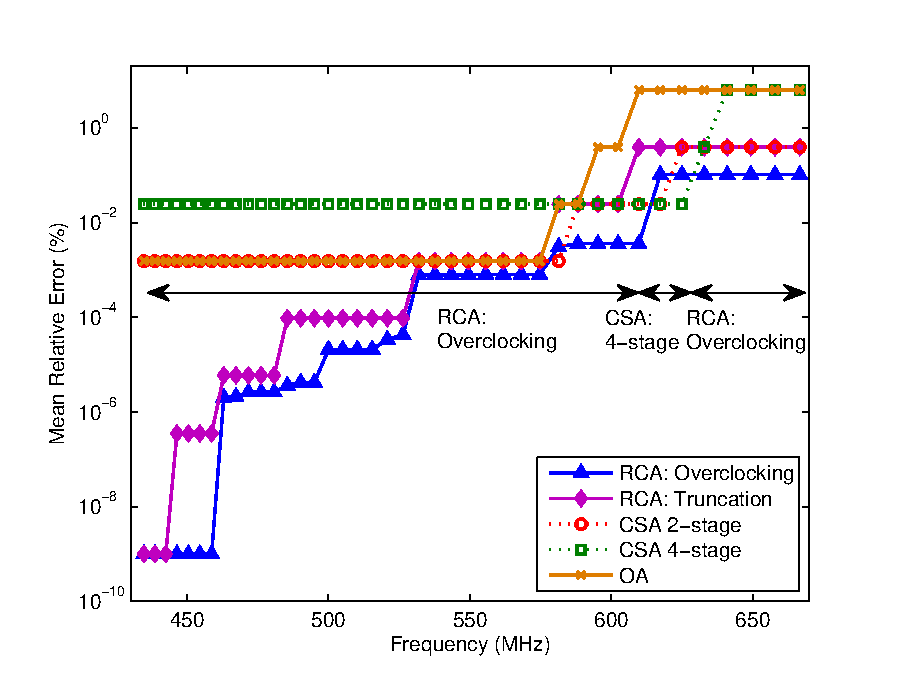
\includegraphics[width=\textwidth]{./figures/exp/Error_LUT35.eps}
    \label{subfig:error_area_lut35}
    \vspace{-2ex}
  \end{minipage}%
  }
  \subfigure[Available LUT=55.]{
  \begin{minipage}[c]{0.5\textwidth}
    \centering
    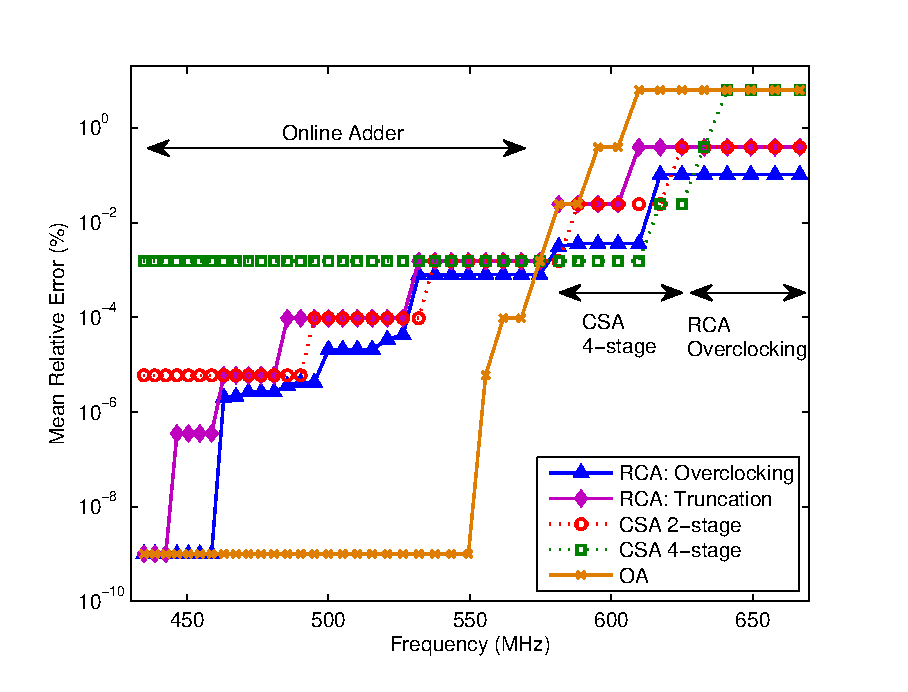
\includegraphics[width=\textwidth]{./figures/exp/Error_LUT55.eps}
    \label{subfig:error_area_lut55}
    \vspace{-2ex}
  \end{minipage}
  }
\caption{Two examples of comparisons between different design scenarios and adder implementations with limited area budget. RCA is evaluated with both overclocking and truncation scenario, whereas CSA and OA are evaluated with truncation scenario only. Design scenario with minimum error is labeled.}
\label{Fig:Error_Area}
%\vspace{-2ex}
\end{figure}

If the area budget is 35 LUTs, as seen in Fig.~\ref{subfig:error_area_lut35}, it can be noticed that for all frequency values, the overcloced RCA achieves no larger mean error than the RCA with truncated operand word-lengths. This is in accordance with the analysis in Section~xxx. We also notice that both CSA and OA cannot be implemented with full precision due to the limited area budget, and this leads to large truncation errors. Despite that the CSA with 4 stages is best for some frequencies, in general the overclocked RCA is still the optimum design for most frequency requirements.  

However if the area budget is released to 55 LUTs, OA can be implemented with original word-length. Additionally CSA can be implemented with larger precision, but still not the full precision. Therefore as shown in Fig.~\ref{subfig:error_area_lut55}, OA serves as the optimum design choice with respect to a wide range of frequencies. For higher frequencies, the MRE of OA increases rapidly, and CSA with 4 stages outperforms for higher frequencies. Similar to Fig.~\ref{subfig:error_area_lut35}, the overclocked RCA is the optimum design choice for even higher frequencies, because in this case the CSA can only be implemented with small precisions, and the multiplexer delay limits the benefits of parallelism.

The results shown in Fig.~\ref{Fig:Error_Area} can be generalized with a variety of area constraints. In this case, the optimum design methods with respect to different operating frequencies and area consumptions are illustrated in Fig.~\ref{Fig:adder_3d_FreqArea}. 
%
\begin{figure*}[tbp]
  \centering
  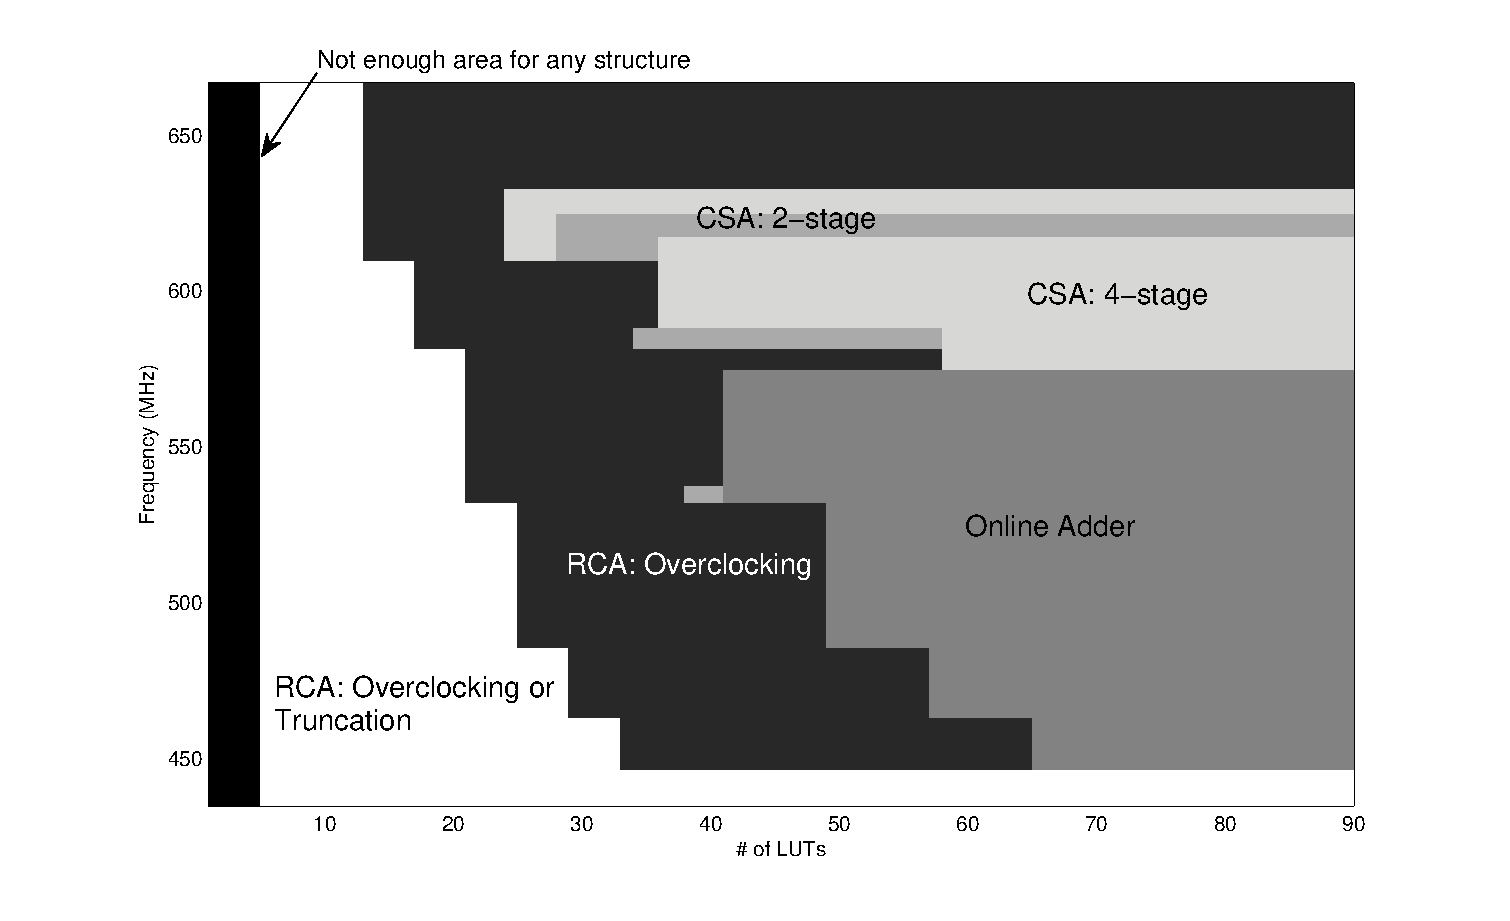
\includegraphics[width=.8\textwidth]{./figures/exp/3d_FreqArea.eps}
  \caption{The maximum word-length of different adder structures.}
  \label{Fig:adder_3d_FreqArea}
\end{figure*}

\subsection{Optimum Adder Design Metric with Given Accuracy and Area Requirements}
%
\begin{figure*}[tbp]
  \centering
  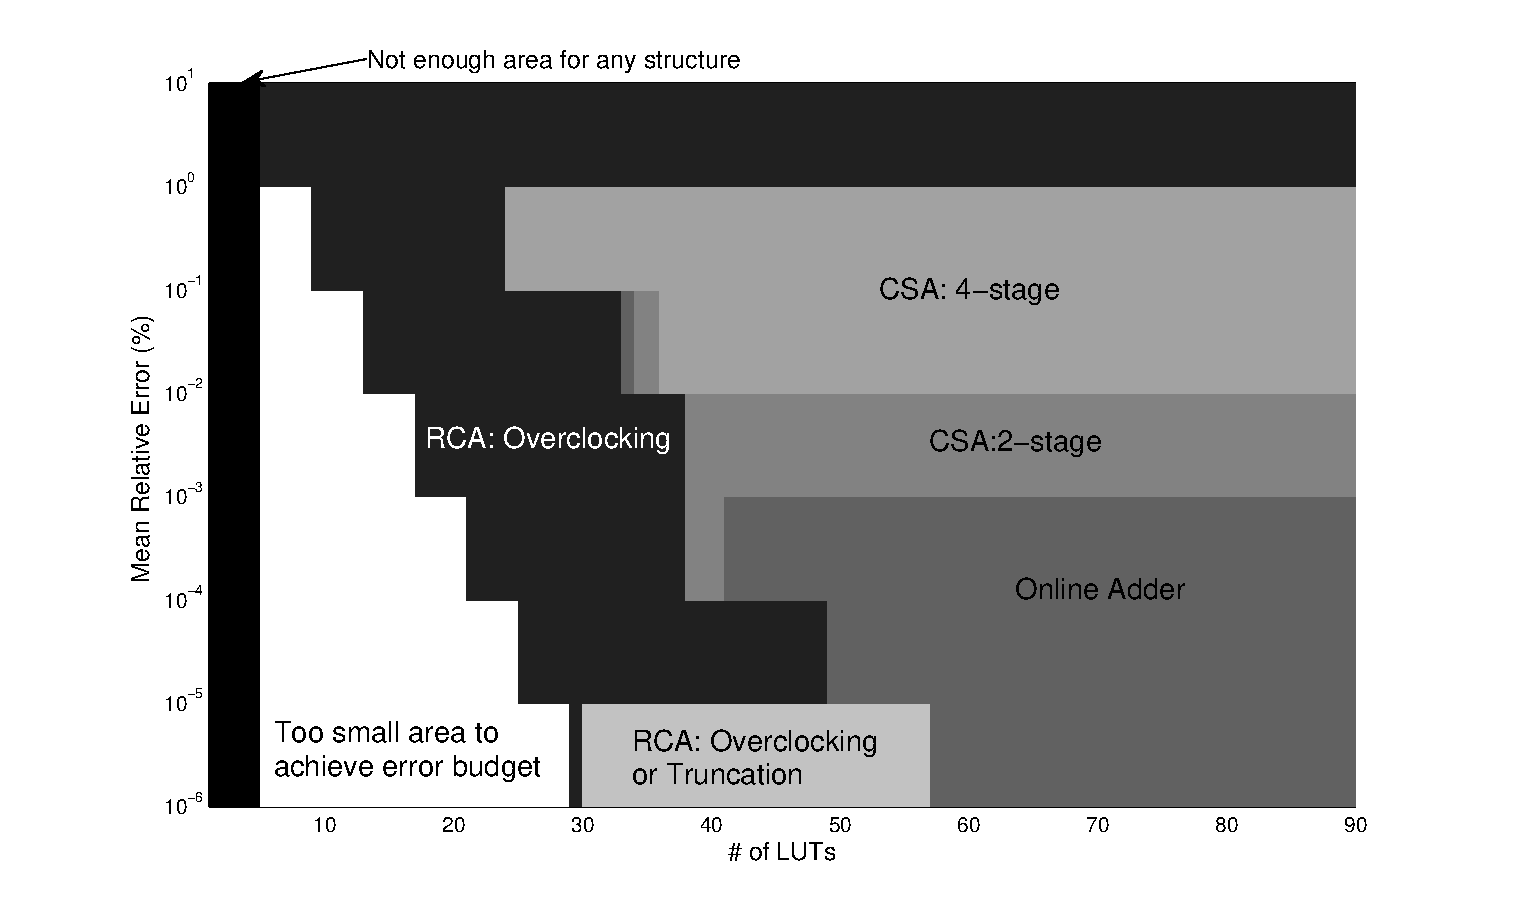
\includegraphics[width=.8\textwidth]{./figures/exp/3d_ErrorArea.eps}
  \caption{The maximum word-length of different adder structures.}
  \label{Fig:adder_3d_ErrorArea}
\end{figure*}

\section{Conclusion}

\section*{Acknowledgment}


\bibliographystyle{./IEEEtran}

\bibliography{./IEEEabrv,./Reference}


\end{document}


